\documentclass[thesis.tex]{subfiles}
\chapter{Mô hình xác minh người nói tiếng Việt}
Trong chương này, tác giả điểm qua các kiên cứu liên quan, trình bày mô hình học sâu cơ sở giải quyết bài toán nhận diện người nói và đề xuất phương pháp để cải tiến mô hình hiện tại để đạt được kết quả cao hơn trên tiếng Việt.

\section{Mô hình cơ sở cho tiếng Anh}\label{baseline}
Mô hình tác giả sử dụng trong đồ án tuân theo hệ thống ba pha được mô tả như trong \ref{related-works}, đây là sự kết hợp giữa mô hình ResNet-34, lớp tổng hợp thống kê tập trung (attentive statistic pooling - ASP) và hàm mất mát Angular Prototypical (AP). Kiến trúc của mô hình được miêu tả trong Hình \ref{fig:ap-resnet}. 

\begin{figure}[h]
    \centering
    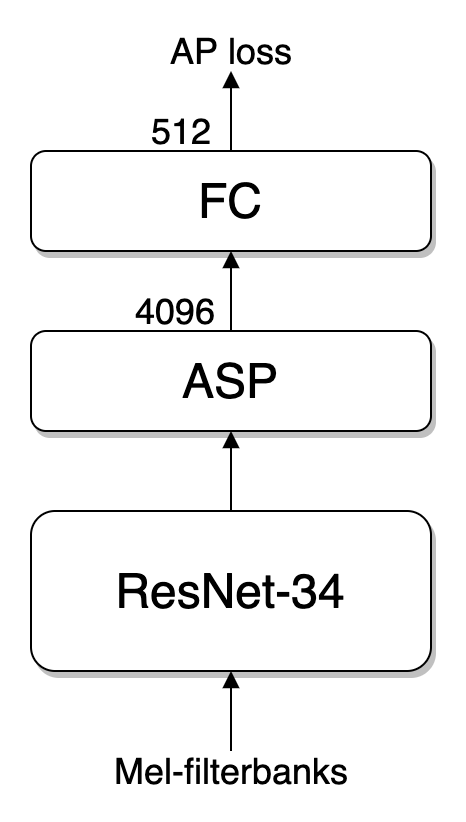
\includegraphics[width=0.4\textwidth]{images/ap-resnet.png}
    \caption{Tổng quan mô hình cơ sở sử dụng trong đồ án}
    \label{fig:ap-resnet}
\end{figure}

Trong các mục tiếp theo, tác giả sẽ trình bày chi tiết thành phần của mô hình.

\subsection{Biểu diễn khung âm thanh bằng mạng ResNet}
Mạng ResNet sử dụng trong đồ án là biến thể của mạng ResNet-34 như mô tả trong hình \ref*{fig:resnet-architecture}. Tại mỗi lớp, mạng sử dụng một nửa số bộ lọc so với mạng ResNet-34 gốc trong các khối ResNet và chứa tổng cộng 8.0 triệu trọng số. Trong lớp tích chập đầu tiên, tham số bước nhảy được chỉnh thành 1 so với 2 trong mạng ResNet-34 gốc khiến đầu vào của các lớp đằng sau lớn hơn từ đó tăng khối lượng tính toán. Chi tiết cấu trúc của mạng được mô tả trong Bảng \ref*{tab:resnet-34}.

\begin{table}[h]
    \centering
    \begin{tabular}{l c c c}
      \hline
      \textbf{Layer}& \textbf{Kernel size} & \textbf{Stride} & \textbf{Output shape} \\
      \hline
      Conv1       & $3 \times 3 \times 32$   & 1 $\times$ 1  & $L \times 64 \times 32$ \\
      \hline
      ResBlock1   & $3 \times 3 \times 32$   & 1 $\times$ 1  & $L \times 64 \times 32$ \\
      \hline
      ResBlock2   & $3 \times 3 \times 64$  & 2 $\times$ 2   & $L/8 \times 32 \times 64$ \\
      \hline
      ResBlock3   & $3 \times 3 \times 128$  & 2 $\times$ 2  & $L/8 \times 16 \times 128$ \\
      \hline
      ResBlock4   & $3 \times 3 \times 256$  & 2 $\times$ 2  & $L/8 \times 8 \times 256$ \\
      \hline
      Flatten     & -  & -  & $L/8 \times 2048$ \\
      \hline
    \end{tabular}
    \caption{Kiến trúc mạng ResNet sử dụng trong đồ án}
    \label{tab:resnet-34}
\end{table}

\subsection{Tổng hợp thống kê tập trung}
Trong thực tế, không phải khung âm thanh nào cũng chứa nhiều thông tin của người nói do độ dài một khung rất ngắn thông thường chỉ 25 mili giây. Ví dụ, một khung có thể chứa nhiều tiếng ồn, hoặc không hề chứa giọng nói. Do vậy, hệ thống sử dụng tổng hợp thống kê tập trung để đánh trọng số cho biểu diễn của các khung với mong muốn tăng thông tin của những khung nhiều ý nghĩa và giảm thông tin của những khung ít ý nghĩa. Từ đó có thể phân biệt giọng nói một cách hiệu quả hơn.
% Được đề xuất bởi Okabe và cộng sự trong \cite{okabe2018attentive}, tổng hợp thống kê tập trung là sự kết hợp giữa tổng hợp thống kê \cite{snyder2018x} và cơ chế tập trung (attention mechanism) \cite{raffel2015feed}.

ASP nhận đầu vào là tập các vec-tơ biểu diễn khung $\bm{h}_t\ (t=1,...,T)$. Vec-tơ biểu diễn của toàn đoạn âm thanh được tính qua 2 bước: đánh trọng số cho từng khung bằng cơ chế tập trung và tổng hợp thông tin thống kê dựa trên trọng số tính được (Hình \ref{fig:asp}).

\begin{figure}[h]
    \centering
    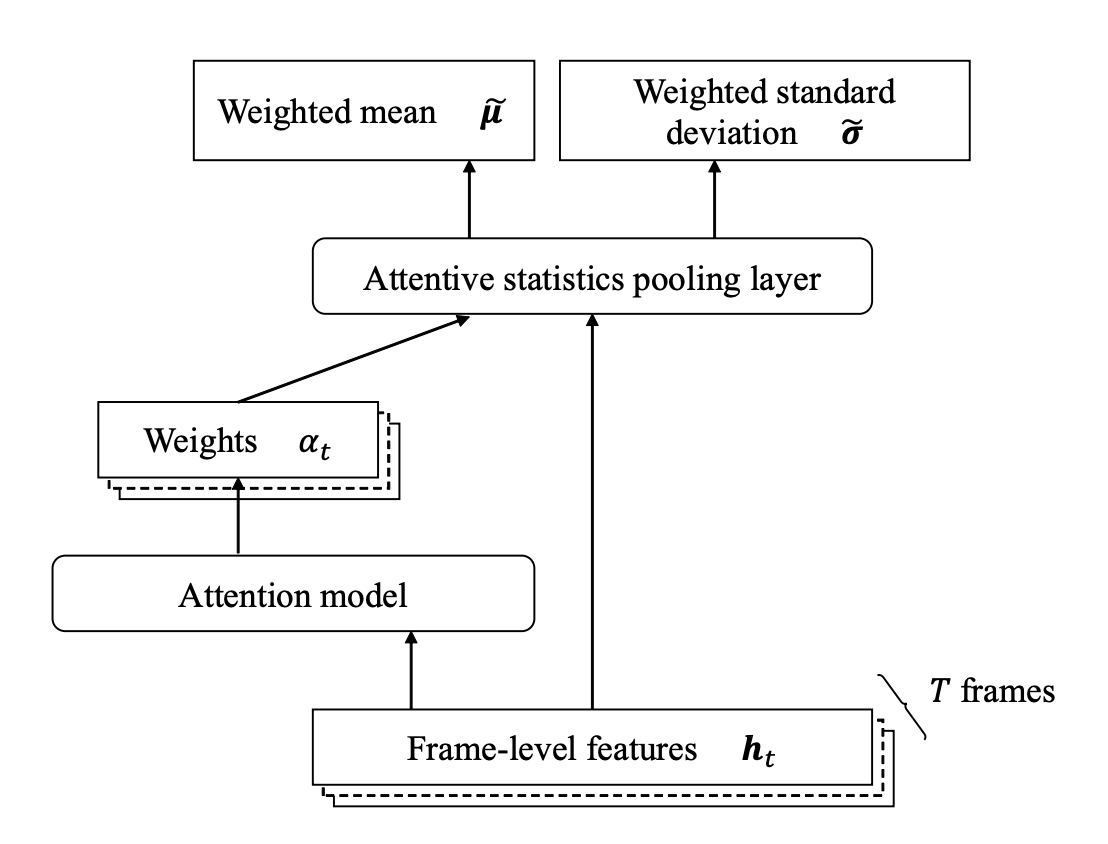
\includegraphics[width=0.7\textwidth]{images/attentive-statistic-pooling.png}
    \caption{Tổng hợp thống kê tập trung \cite{okabe2018attentive}}
    \label{fig:asp}
\end{figure}

\subsubsection{Cơ chế tập trung}

Bằng cơ chế tập trung, trọng số của từng khung có thể được tính như sau: 

\begin{equation} \label{eq:att1}
    e_t = \bm{v}^T f(\bm{W}\bm{h}_t + b) + k
\end{equation}

\begin{equation} \label{eq:att2}
    \alpha_t = \dfrac{\alpha_t}{\sum_\rho^T \alpha_\rho}
\end{equation}

Trong công thức \ref{eq:att1}, với $\bm{v}, \bm{W}$ là các ma trận trọng số có thể học được, $f$ là hàm phi tuyến như thanh hoặc ReLu, ta tính được điểm cho mỗi khung $e_t$. Sau đó, điểm của mỗi khung được chuẩn hoá trên tất cả các khung để thu được trọng số tập trung bằng hàm softmax như trong \ref{eq:att2}.

\subsubsection{Tổng hợp thống kê}
Sau khi có được trọng số của các khung, ta tính vec-tơ trung bình có trọng số:

\begin{equation} \label{eq:asp1}
    \bm{\mu} = \sum_t^T \alpha_t\ \bm{h}_t
\end{equation}

Bằng cách tính này, vec-tơ biểu diễn của đoạn âm thanh tập trung hơn vào những khung tiếng nói có ý nghĩa cao. Ngoài ra, các trọng số tập trung còn được sử dụng để tính độ lệch chuẩn có trọng số:

\begin{equation} \label{eq:asp2}
    \bm{\sigma} = \sqrt{\sum_t^T \alpha_t \bm{h}_t \odot \bm{h}_t - \bm{\mu} \odot \bm{\mu}}
\end{equation}

Với $\odot$ là phép nhân Hadamard, $\bm{\mu}$ là vec-tơ trung bình có trọng số tính trong công thức \ref{eq:asp1}. Sau khi hoàn tất quá trình tính toán vec-tơ trung bình và độ lệch chuẩn có trọng số, $\bm{\mu}$ và $\bm{\sigma}$ được ghép lại để biểu diễn cho một đoạn tiếng nói. Bằng cách này, mọi đoạn âm thanh dài ngắn đều có vec-tơ biểu diễn với số chiều như nhau, được tổng hợp từ những khung âm thanh có ý nghĩa nhất trong câu.

\subsection{Hàm mất mát Angular Prototypical} \label{ap-loss}
Trong thực tế, ta cần tổng hợp từ một số câu nói nhất định để tạo vec-tơ biểu diễn người nói. Do vậy, Chung và cộng sự \cite{chung2020defence} đề xuất hàm mất mát AP tối ưu không gian biểu diễn dựa trên nguyên mẫu (prototype) của người nói. Mỗi người nói có một nguyên mẫu và một câu truy vấn, mục tiêu của AP là đẩy xa truy vấn của một người ra xa nguyên mẫu của những người khác và kéo nó lại gần nguyên mẫu của người đó (Hình \ref{fig:ap-loss}).

\begin{figure}[h]
    \centering
    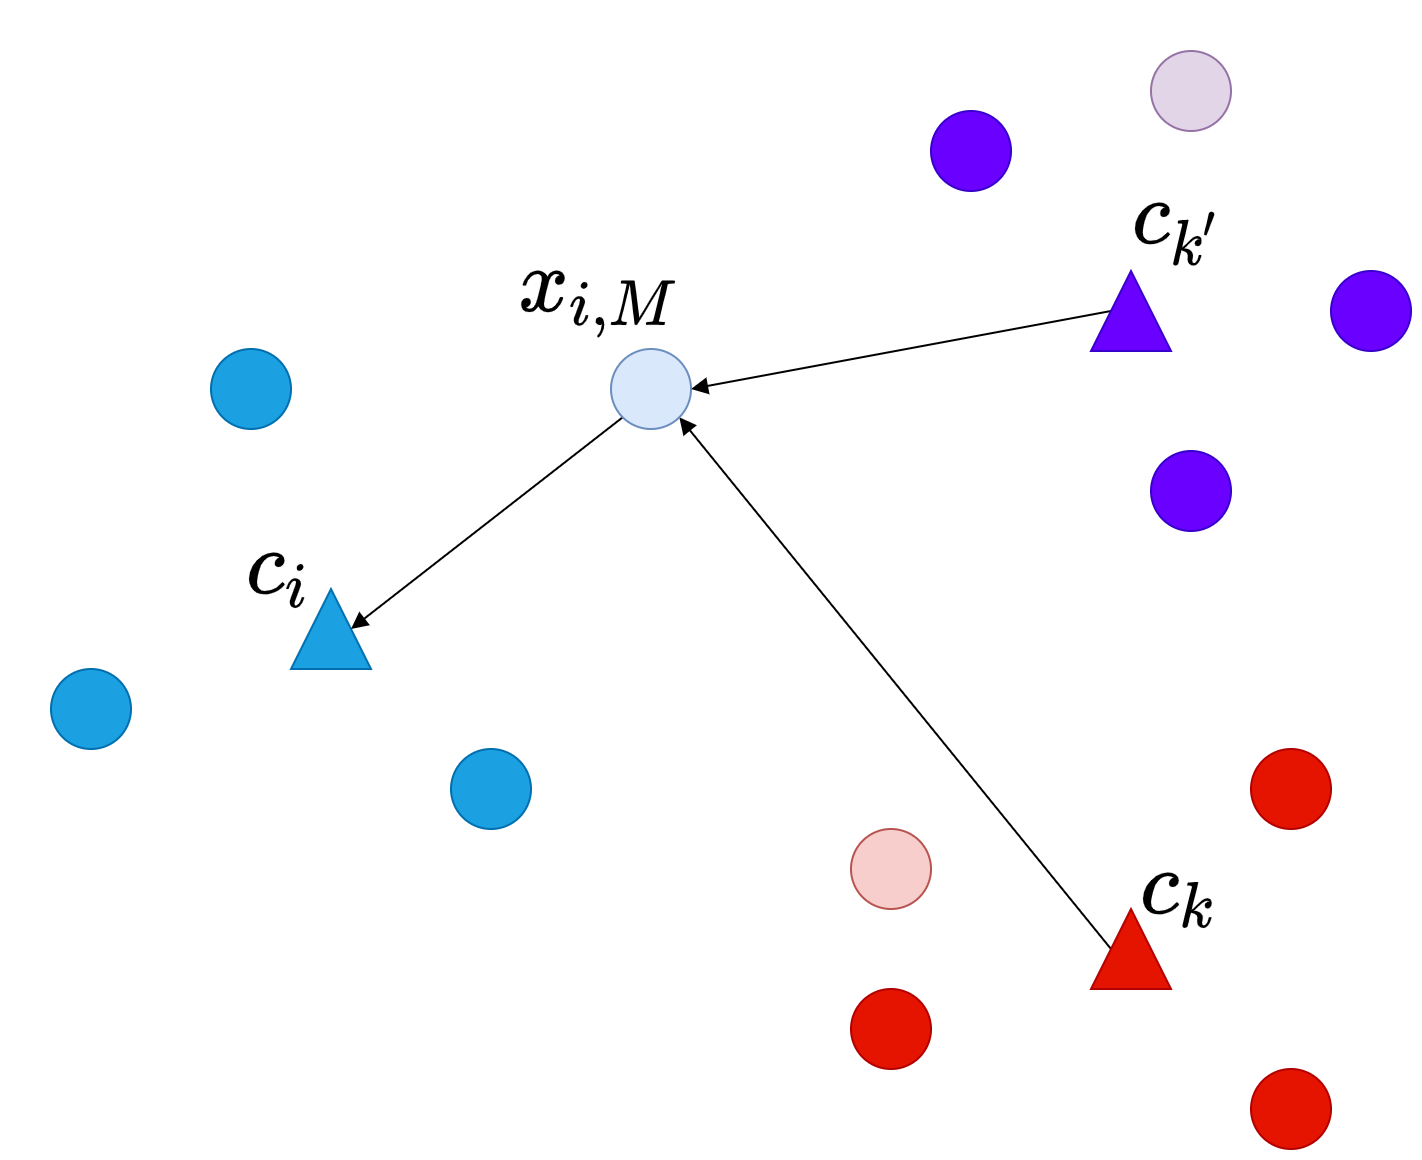
\includegraphics[width=0.7\textwidth]{images/ap-loss.png}
    \caption{Hàm mất mát Angular Prototypical}
    \label{fig:ap-loss}
\end{figure}

Xét một mini-batch gồm $M$ đoạn tiếng nói từ mỗi $N$ người nói, gọi $\bm{x}_{i,j}$ là vec-tơ biểu diễn của đoạn tiếng nói thứ $j$ của người thứ $i$, $1 \leq i \leq N, 1 \leq j \leq M$. Giả sử truy vấn của một người là câu cuối cùng của người đó $\bm{x}_{i,M}$, nguyên mẫu của một người nói được tính toán như sau:

\begin{equation}
    \bm{c}_i = \dfrac{1}{M-1}\sum_{m=1}^{M-1}\ \bm{x}_{i,m}
\end{equation}

Trong AP, độ tương đồng cô-sin được sử dụng để làm độ đo. Độ tương đồng được tính theo công thức \ref{eq:cosine} với hệ số scale $w$ và bias $b$. Hai hệ số này giúp mô hình hội tụ ổn định hơn và khái quát hoá tốt hơn với thay đổi trong đặc trưng đầu vào \cite{wang2017deep}.

\begin{equation}\label{eq:cosine}
    \bm{S}_{i,k} = w \cdot cos(\bm{x}_{i,M}, \bm{c}_k) + b
\end{equation}

Trong quá trình huấn luyện, câu truy vấn của mỗi người được phân loại dựa trên độ tương đồng đối với $N$ nguyên mẫu trong mini-batch:

\begin{equation}\label{eq:nll-softmax}
    L_{AP} = - \dfrac{1}{N} \sum_{i=1}^N log \dfrac{e^{\bm{S}_{i,i}}}{\sum_{k=1}^N e^{\bm{S}_{i,k}}}
\end{equation}

Trong công thức \ref*{eq:nll-softmax}, $\bm{S}_{i, i}$ là độ tương đồng của truy vấn người $i$ và nguyên mẫu của chính người đó. Bằng việc sử dụng hàm softmax, $\bm{S}_{i,i}$ được đẩy gần hơn tới 1 và mô hình bị "phạt" nặng hơn nếu độ tương đồng của truy vấn người $i$ tới nguyên mẫu của người khác lớn.

\section{Đề xuất mô hình cho tiếng Việt}
\subsection{Mô hình tổng quan}

Trong phần này, nhận thấy một vài điểm chưa được tối ưu trong mô hình cơ sở, tác giả đề xuất các phương pháp giúp huấn luyện mô hình một cách có hiệu quả hơn bao gồm: học chuyển tiếp (transfer learning), hàm tối ưu SGD thay cho Adam trong mô hình cơ sở, thêm hệ số phạt góc cho hàm mất mát AP (Hình \ref{fig:overall-propose}). Các mục dưới trình bày chi tiết các phương pháp đề xuất.

\begin{figure}[h]
    \centering
    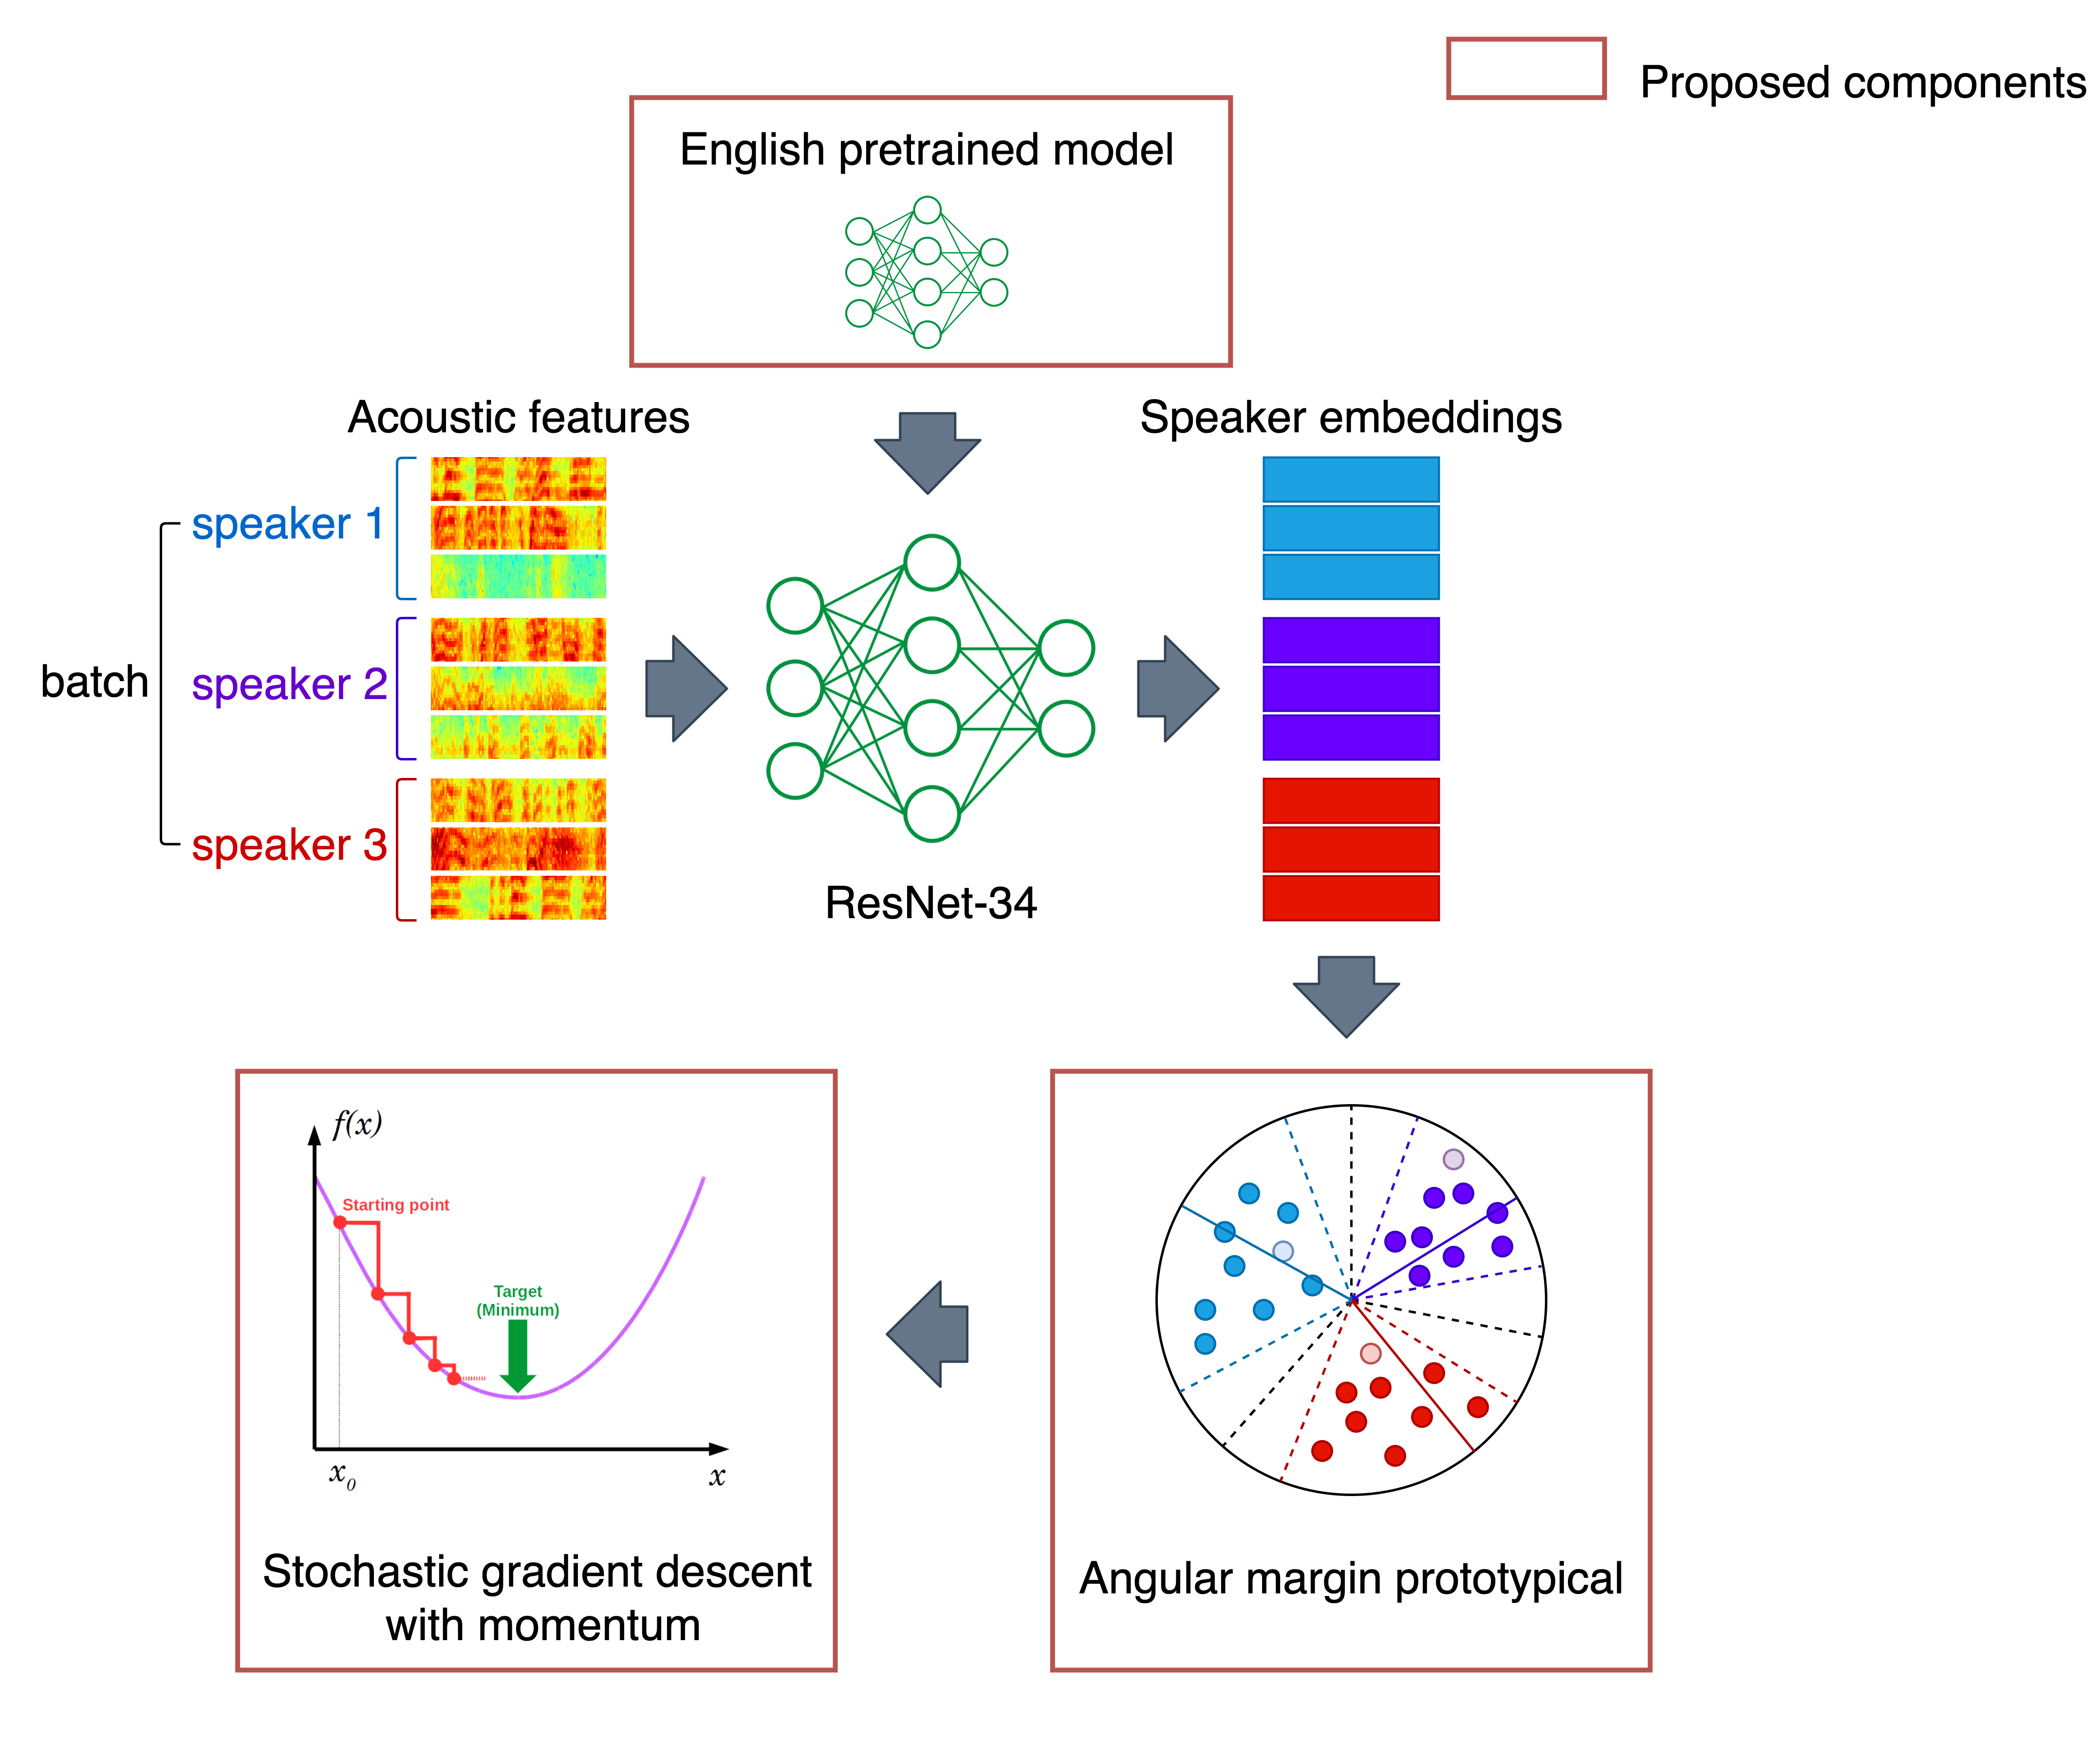
\includegraphics[width=1\textwidth]{images/overall-propose.png}
    \caption{Tổng quan phương pháp đề xuất cho nhận dạng người nói tiếng Việt}
    \label{fig:overall-propose}
\end{figure}

\subsection{Học chuyển tiếp}
Học chuyển tiếp là một kỹ thuật trong học máy khi mà một mô hình được huấn luyện cho một tác vụ nhất định được sử dụng làm điểm bắt đầu cho một tác vụ khác. Học chuyển tiếp cho phép rút ngắn quá trình huấn luyện và gia tăng hiệu năng cho quá trình huấn luyện mô hình trên tác vụ mới với ít dữ liệu hơn đáng kể. 

\begin{figure}[h]
    \centering
    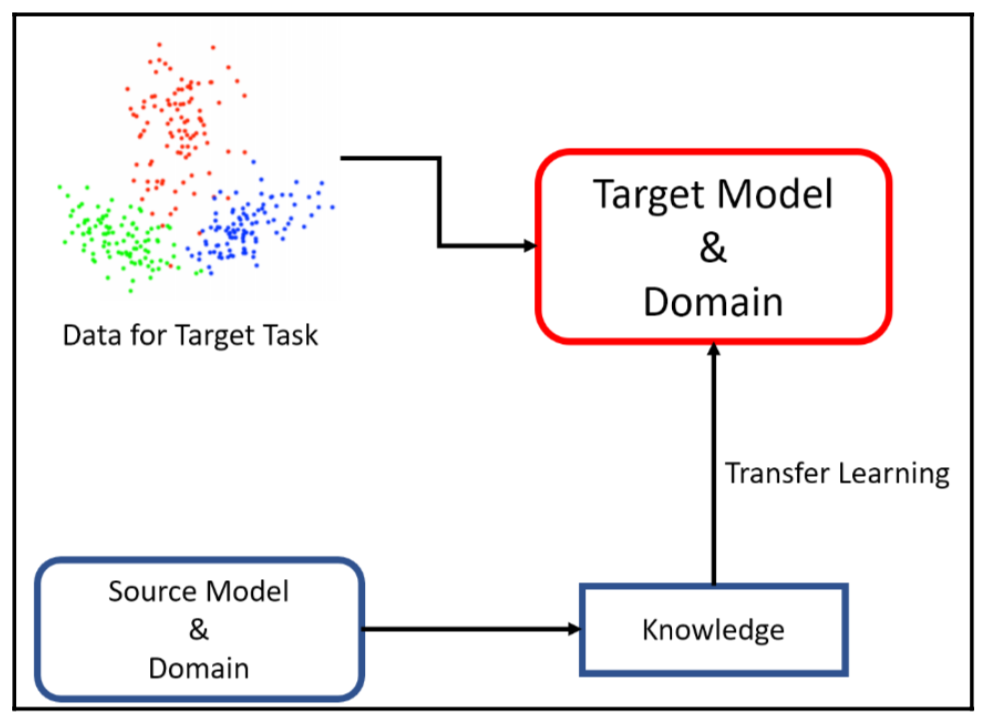
\includegraphics[width=0.7\textwidth]{images/transfer-learning.png}
    \caption{Sơ đồ mô tả học chuyển tiếp sử dụng kiến thức hiện có cho các tác vụ mới \cite{sarkar2018hands}}
    \label{fig:transfer-learning}
\end{figure}

Cụ thể hơn, học chuyển tiếp hỗ trợ việc huấn luyện tác vụ mục tiêu theo những cách sau: 

\begin{itemize}
    \item Hiệu suất cơ sở tốt hơn (higher start): khi ta tăng cường kiến thức của mô hình mới với kiến thức từ mô hình gốc, hiệu suất cơ sở có thể cải thiện nhờ việc chuyển giao kiến thức.
    \item Thời gian huấn luyện ngắn hơn (higher slope): tốc độ hội tụ của mô hình mới có thể nhanh hơn dẫn tới thời gian huấn luyện ngắn hơn.
    \item Kết quả cuối cùng tốt hơn (higher asymptote): hiệu suất cuối cùng cao hơn có thể đạt được bằng việc sử dụng học chuyển tiếp.
\end{itemize}

\begin{figure}[h]
    \centering
    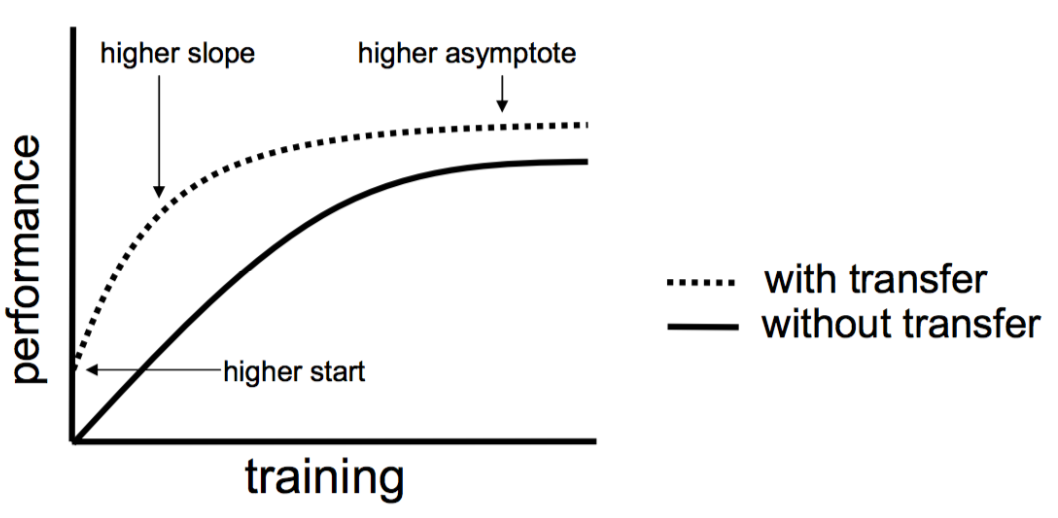
\includegraphics[width=0.7\textwidth]{images/transfer-learning-benefits.png}
    \caption{Lợi ích của học chuyển tiếp đối với việc huấn luyện mô hình \cite{aytar2011tabula}}
    \label{fig:transfer-learning-benefits}
\end{figure}

Huấn luyện mô hình học sâu cần một lượng lớn tài nguyên tính toán và dữ liệu, do đó học chuyển tiếp được sử dụng rộng rãi trong cộng đồng nghiên cứu học sâu cho bài toán thị giác máy tính hay xử lý ngôn ngữ tự nhiên. Các thư viện học sâu nổi tiếng như Pytorch hay Tensorflow đều công bố các mô hình huấn luyện sẵn trên hàng triệu hay chục triệu ảnh giúp cộng đồng phát triển các mô hình học sâu dễ dàng và hiệu quả hơn với ít dữ liệu. Gần đây, cộng đồng nghiên cứu xử lý ngôn ngữ tự nhiên cũng có thể lợi dụng các mô hình huấn luyện sẵn cực lớn với hàng trăm tỉ trọng số như BERT \cite{devlin2018bert}, GPT-2 \cite{radford2019language} hay GPT-3 \cite{brown2020language} để cải tiến các tác vụ hạ lưu như phân loại nhận dạng thực thể, phân tích cú pháp phụ thuộc, tóm tắt văn bản, ...

% Trong nhận dạng người nói, transfer learning cũng được áp dụng \TODO{transfer learning in speaker recognition}. 
Trong đồ án, phương pháp học chuyển tiếp từ mô hình huấn luyện trên người nói tiếng Anh được áp dụng để cải thiện mô hình giọng nói tiếng Việt. 

\subsection{SGD với momentum khái quát hoá tốt hơn Adam}
Adam \cite{kingma2014adam} là một thuật toán tối ưu thích nghi hệ số học. Được công bố vào năm 2014, Adam được trình bày tại một hội nghị rất uy tín cho cộng đồng học sâu - ICLR 2015. Bài báo phát triển một thuật toán rất hứa hẹn, cho thấy sự hội tụ vượt trội so với các thuật toán hiện hành, dẫn đến tăng tốc trong quá trình huấn luyện. 
 
Adam thích nghi hệ số học cho một trọng số của mạng sử dụng giá trị trung bình trượt của gradient và gradient bình phương của trọng số đó qua các mini-batch. Cho các trọng số $w^{(t)}$ và hàm mất mát $L^{(t)}$, trong đó $t$ là chỉ số vòng lặp trong quá trình huấn luyện, việc cập nhật trọng số trong Adam như sau:

\begin{equation} \label{eq:adam}
    \begin{split}
    m_{w}^{(t+1)} \leftarrow \beta_{1} m_{w}^{(t)}+\left(1-\beta_{1}\right) \nabla_{w} L^{(t)} \\
    v_{w}^{(t+1)} \leftarrow \beta_{2} v_{w}^{(t)}+\left(1-\beta_{2}\right)\left(\nabla_{w} L^{(t)}\right)^{2} \\ 
    \hat{m}_{w}=\frac{m_{w}^{(t+1)}}{1-\beta_{1}^{t+1}} \\ 
    \hat{v}_{w}=\frac{v_{w}^{(t+1)}}{1-\beta_{2}^{t+1}} \\
    w^{(t+1)} \leftarrow w^{(t)}-\eta \frac{\hat{m}_{w}}{\sqrt{\hat{v}_{w}}+\epsilon}
    \end{split}
\end{equation}

trong đó $\epsilon$ là một hệ số cực bé (ví dụ $10^{-6}$) để tránh phép chia cho 0, $\beta_1$ và $\beta_2$ là hệ số quên cho giá trị trung bình trượt bậc 1 và bậc 2 tương ứng. Phương pháp tối ưu đã được sử dụng trong nhiều ứng dụng do hiệu suất cạnh tranh và khả năng hoạt động tốt mà không cần điều chỉnh các hệ số. Công thức \ref*{eq:adam} cho thấy kích thước bước nhảy của quy tắc cập nhật trong Adam bất biến với độ lớn của gradient.

Tuy nhiên sau một thời gian, cộng đồng bắt đầu nhận thấy trong một số trường hợp, Adam huấn luyện mô hình tệ hơn so với phương pháp tối ưu truyền thống SGD. Bằng thực nghiệm, nghiên cứu \cite{keskar2017improving} cho thấy Adam dù trong những vòng lặp đầu vượt trội so với SGD ở những vòng lặp đầu nhưng nhanh chóng trì trệ trong những vòng lặp sau. Wilson cùng cộng sự trong \cite{wilson2017marginal} chỉ ra rằng các phương pháp thích ứng như Adam hay Adadelta không khái quát hoá SGD với momentum sau khi thử nghiệm trên một loạt các tác vụ, không khuyến khích cộng đồng sử dụng các thuật toán thích ứng. Nhìn chung, các nghiên cứu cho thấy rằng tính tổng quá hoá của Adam tệ hơn SGD.

Trong bài toán nhận diện người nói, người nói trong pha kiểm tra thường không có trong tập huấn luyện, tính tổng quát hoá của mô hình là đặc biệt quan trọng. Lý do chính là bởi vì môi trường trong pha kiểm thử khác nhau rất nhiều so với môi trường trong dữ liệu huấn luyện và đăng ký. Do vậy mô hình có tính tổng quát hoá cao, nghĩa là ít nhạy cảm với điều kiện của môi trường cho kết quả tốt hơn.

Vì các lý do kể trên, đồ án đề xuất thay thế sử dụng SGD với momentum thay cho Adam trong mô hình cơ sở.

\subsection{Hàm mất mát Angular Margin Prototypical}
Như đã mô tả trong \ref{ap-loss}, hàm mất mát AP khuyến khích biểu diễn câu nói của một người gần hơn tới nguyên mẫu $\bm{c}_i$ của người đó hơn là các nguyên mẫu khác. Tuy vậy, khoảng cách giữa các câu nói của một người còn khá lớn và các câu khác người nói ở gần biên quyết định hàm softmax có khoảng cách nhỏ. Đây cũng là điểm yếu của hàm softmax mà nhiều nghiên cứu trước đây cũng đã chỉ ra. Biên quyết định yếu có thể gây ra tỉ lệ nhầm lẫn cao khi triển khai mô hình trong thực tế.

\begin{figure}[h]
    \centering
    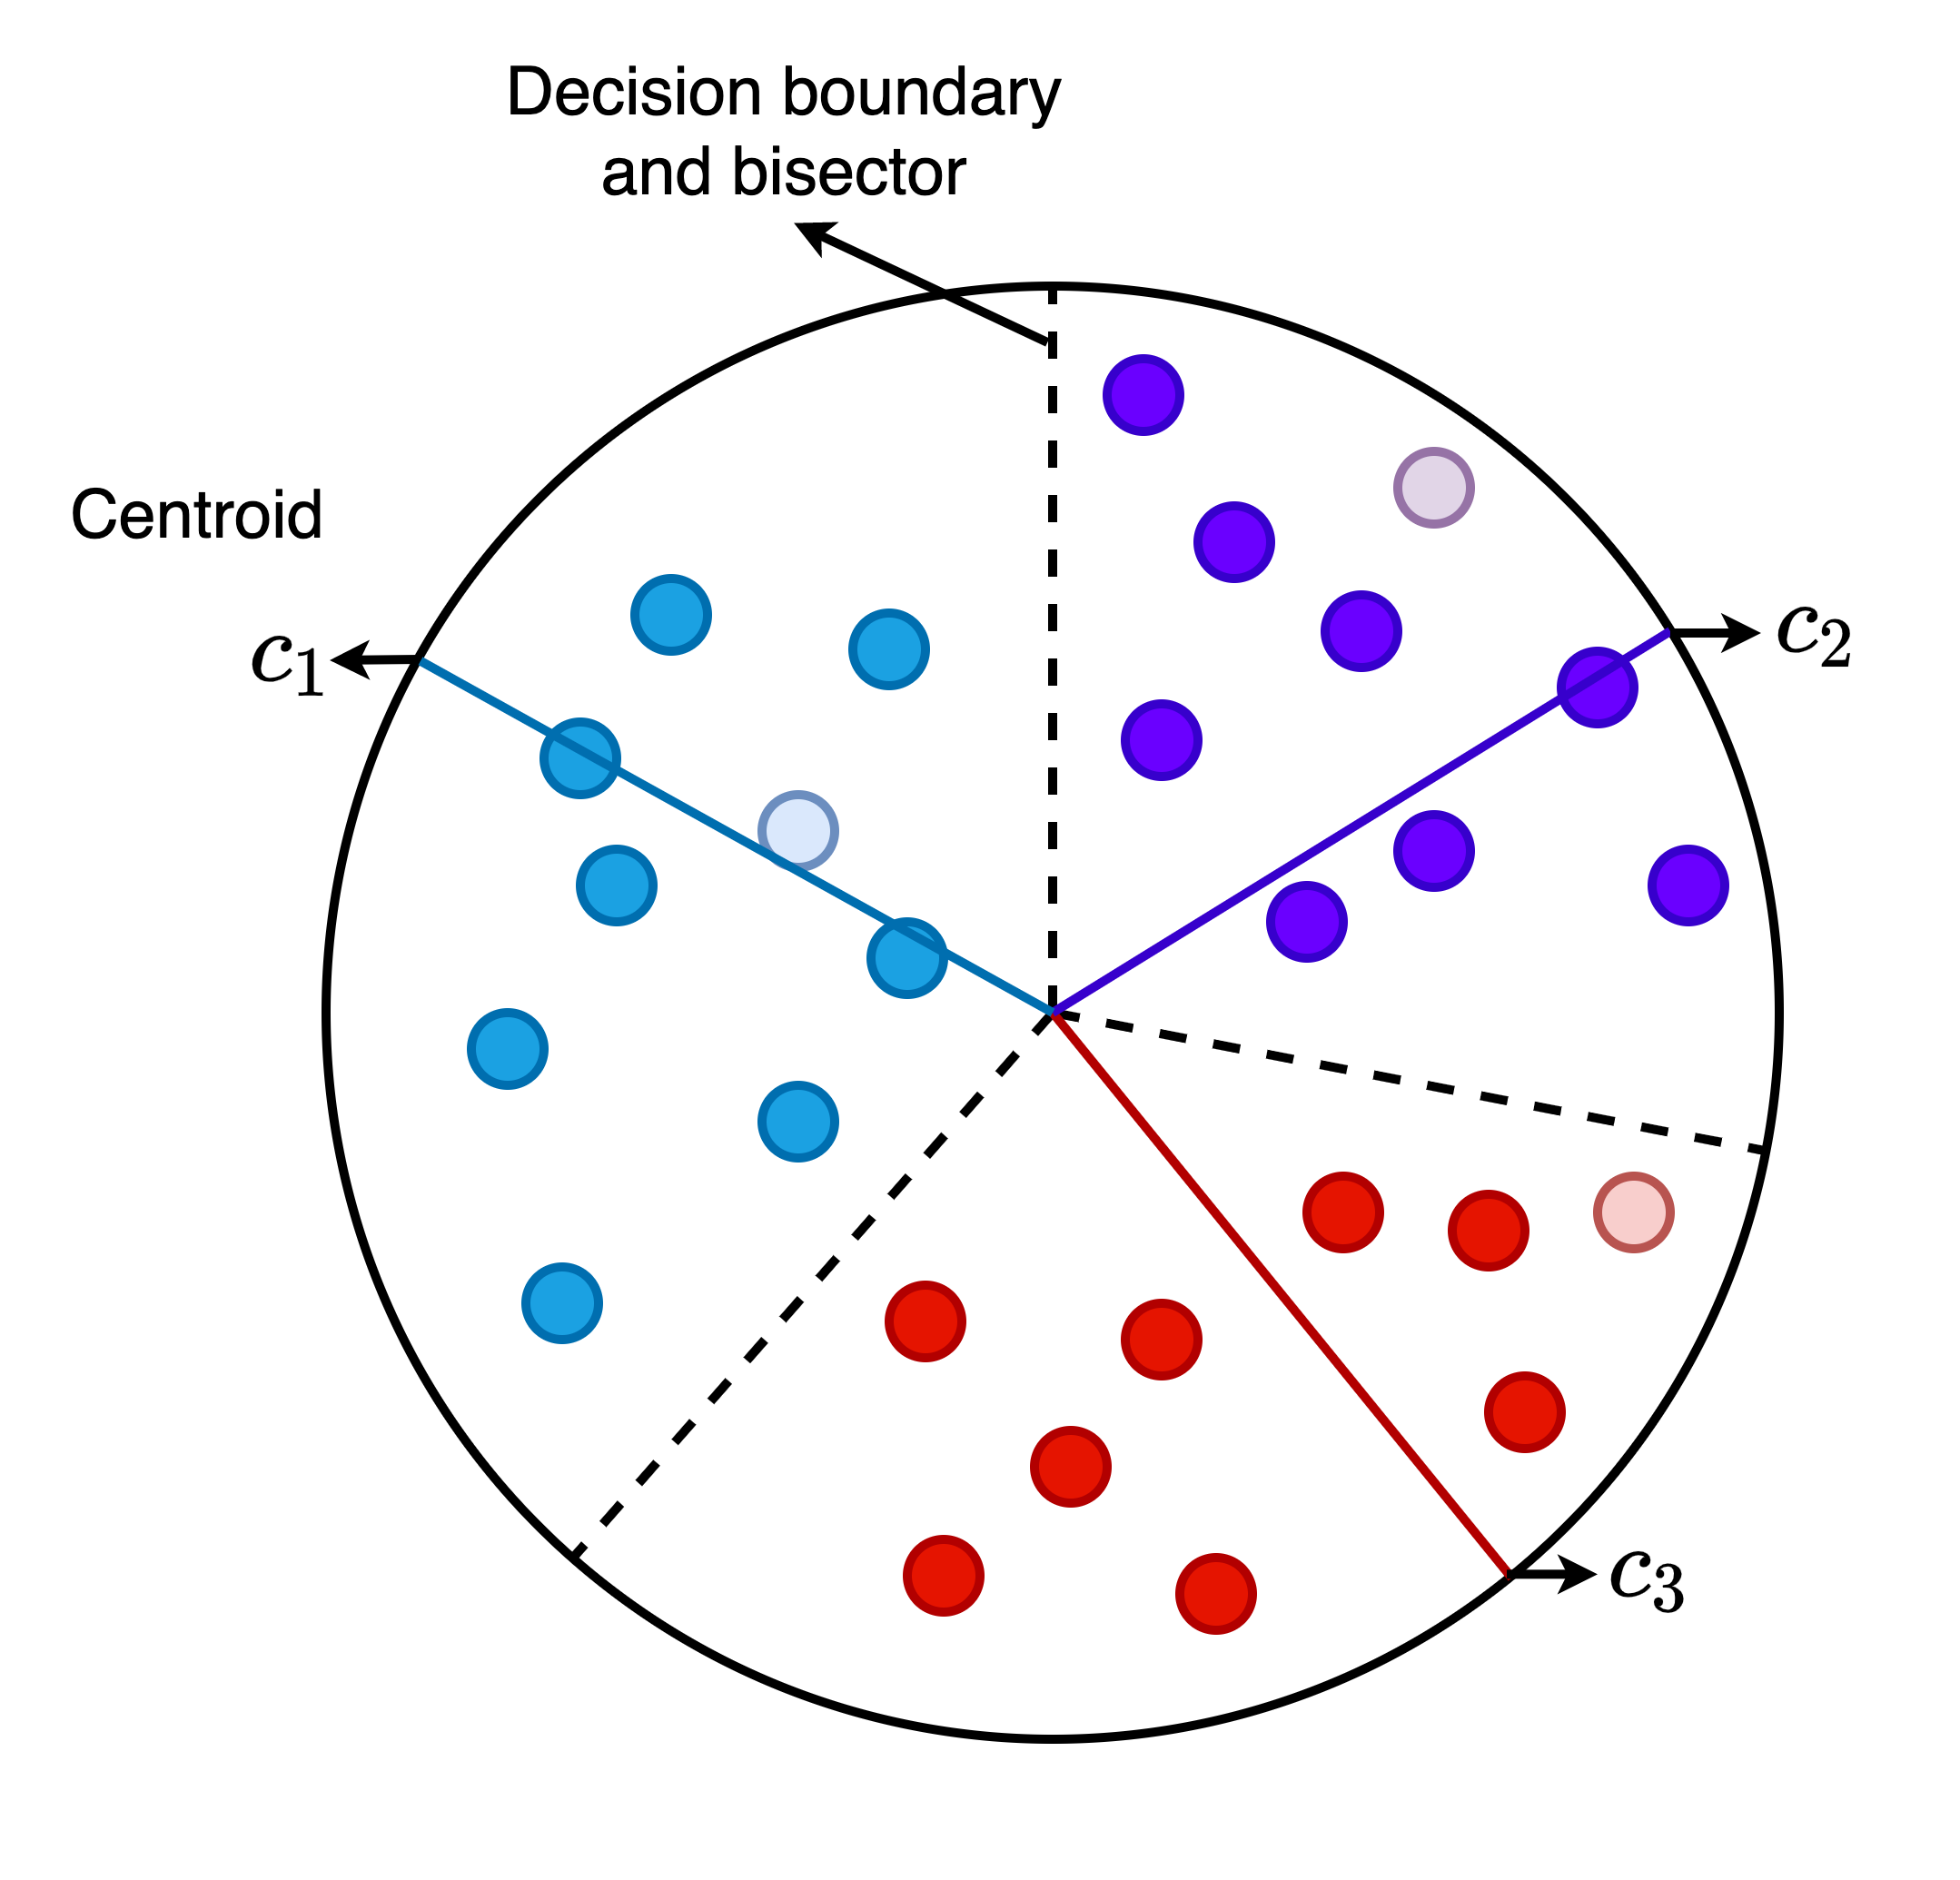
\includegraphics[width=0.54\textwidth]{images/softmax-angular-space.png}
    \caption{Mô tả biểu diễn người nói học bởi hàm softmax trong không gian góc. Đường kẻ chấm đen là đường phân giác giữa 2 tâm}
    \label{fig:softmax-angular-space}
\end{figure}

Nhận thấy sự hiệu quả của việc dùng hệ số phạt lề trong các hàm mất mát phân loại như AM-Softmax \cite{wang2018additive} hay \cite{deng2019arcface}, tác giả đề xuất hàm mất mát Angular Margin Prototypical (AMP) thêm hệ số phạt lề vào hàm AP. Hàm AMP có thể được chia thành 2 loại AMP-cos hoặc AMP-arc phụ thuộc vào cách thêm hệ số phạt vào điểm tương đồng cô-sin hay góc giữa điểm biểu diễn và nguyên mẫu.

\subsubsection{AMP-cos}
Trong hàm AMP-cos, hệ số phạt lề được thêm trực tiếp vào điểm tương đồng của 2 câu. Công thức tính điểm tương đồng \label{eq:cosine} được thay đổi như sau:

\begin{equation}
    \bm{S}_{i, k} = 
\begin{cases}
    w \cdot (\cos \left(\theta_{\bm{x}_{i, M}, \bm{c}_{k}}\right) - m)+b, & \text{if } i = k\\
    w \cdot \cos \left(\theta_{\bm{x}_{i, M}, \bm{c}_{k}}\right)+b,              & \text{otherwise}
\end{cases}
\end{equation}

trong đó $\theta_{\bm{x}_{i, M}, \bm{c}_{k}}$ là góc giữa truy vẫn $\bm{x}_{i, M}$ của người $i$ và nguyên mẫu $\bm{c}_{k}$ của người $k$, $w$ và $b$ là các trọng số học được, và $m$ là hệ số phạt lề. Thay vào công thức \ref{eq:nll-softmax}, ta được hàm mất mát AMP-cos như sau:

\begin{equation}
    L_{AMP-cos} = - \dfrac{1}{N} \sum_{i=1}^N log \dfrac{e^{w \cdot (\cos \left(\theta_{\bm{x}_{i, M}, \bm{c}_{i}}\right) - m)+b}}{e^{w \cdot (\cos \left(\theta_{\bm{x}_{i, M}, \bm{c}_{i}}\right) - m)+b} + \sum_{k=1, k \neq i}^N e^{w \cdot \cos \left(\theta_{\bm{x}_{i, M}, \bm{c}_{k}}\right)+b}}
\end{equation}

\subsubsection{AMP-arc}
Hệ số phạt lề được thêm vào góc giữa 2 câu trong hàm AMP-arc. Công thức tính điểm tương đồng \label{eq:cosine} được thay đổi như sau:

\begin{equation}
    \bm{S}_{i, k} = 
\begin{cases}
    w \cdot \cos \left(\theta_{\bm{x}_{i, M}, \bm{c}_{k}} + m\right)+b, & \text{if } i = k\\
    w \cdot \cos \left(\theta_{\bm{x}_{i, M}, \bm{c}_{k}}\right)+b,              & \text{otherwise}
\end{cases}
\end{equation}

Thay công thức trên vào \ref{eq:nll-softmax}, ta được hàm mất mát AMP-arc như sau:

\begin{equation}
    L_{AMP-arc} = - \dfrac{1}{N} \sum_{i=1}^N log \dfrac{e^{w \cdot \cos \left(\theta_{\bm{x}_{i, M}, \bm{c}_{i}} + m\right)+b}}{e^{w \cdot \cos \left(\theta_{\bm{x}_{i, M}, \bm{c}_{i}} + m\right)+b} + \sum_{k=1, k \neq i}^N e^{w \cdot \cos \left(\theta_{\bm{x}_{i, M}, \bm{c}_{k}}\right)+b}}
\end{equation}

\begin{figure}[h]
    \centering
    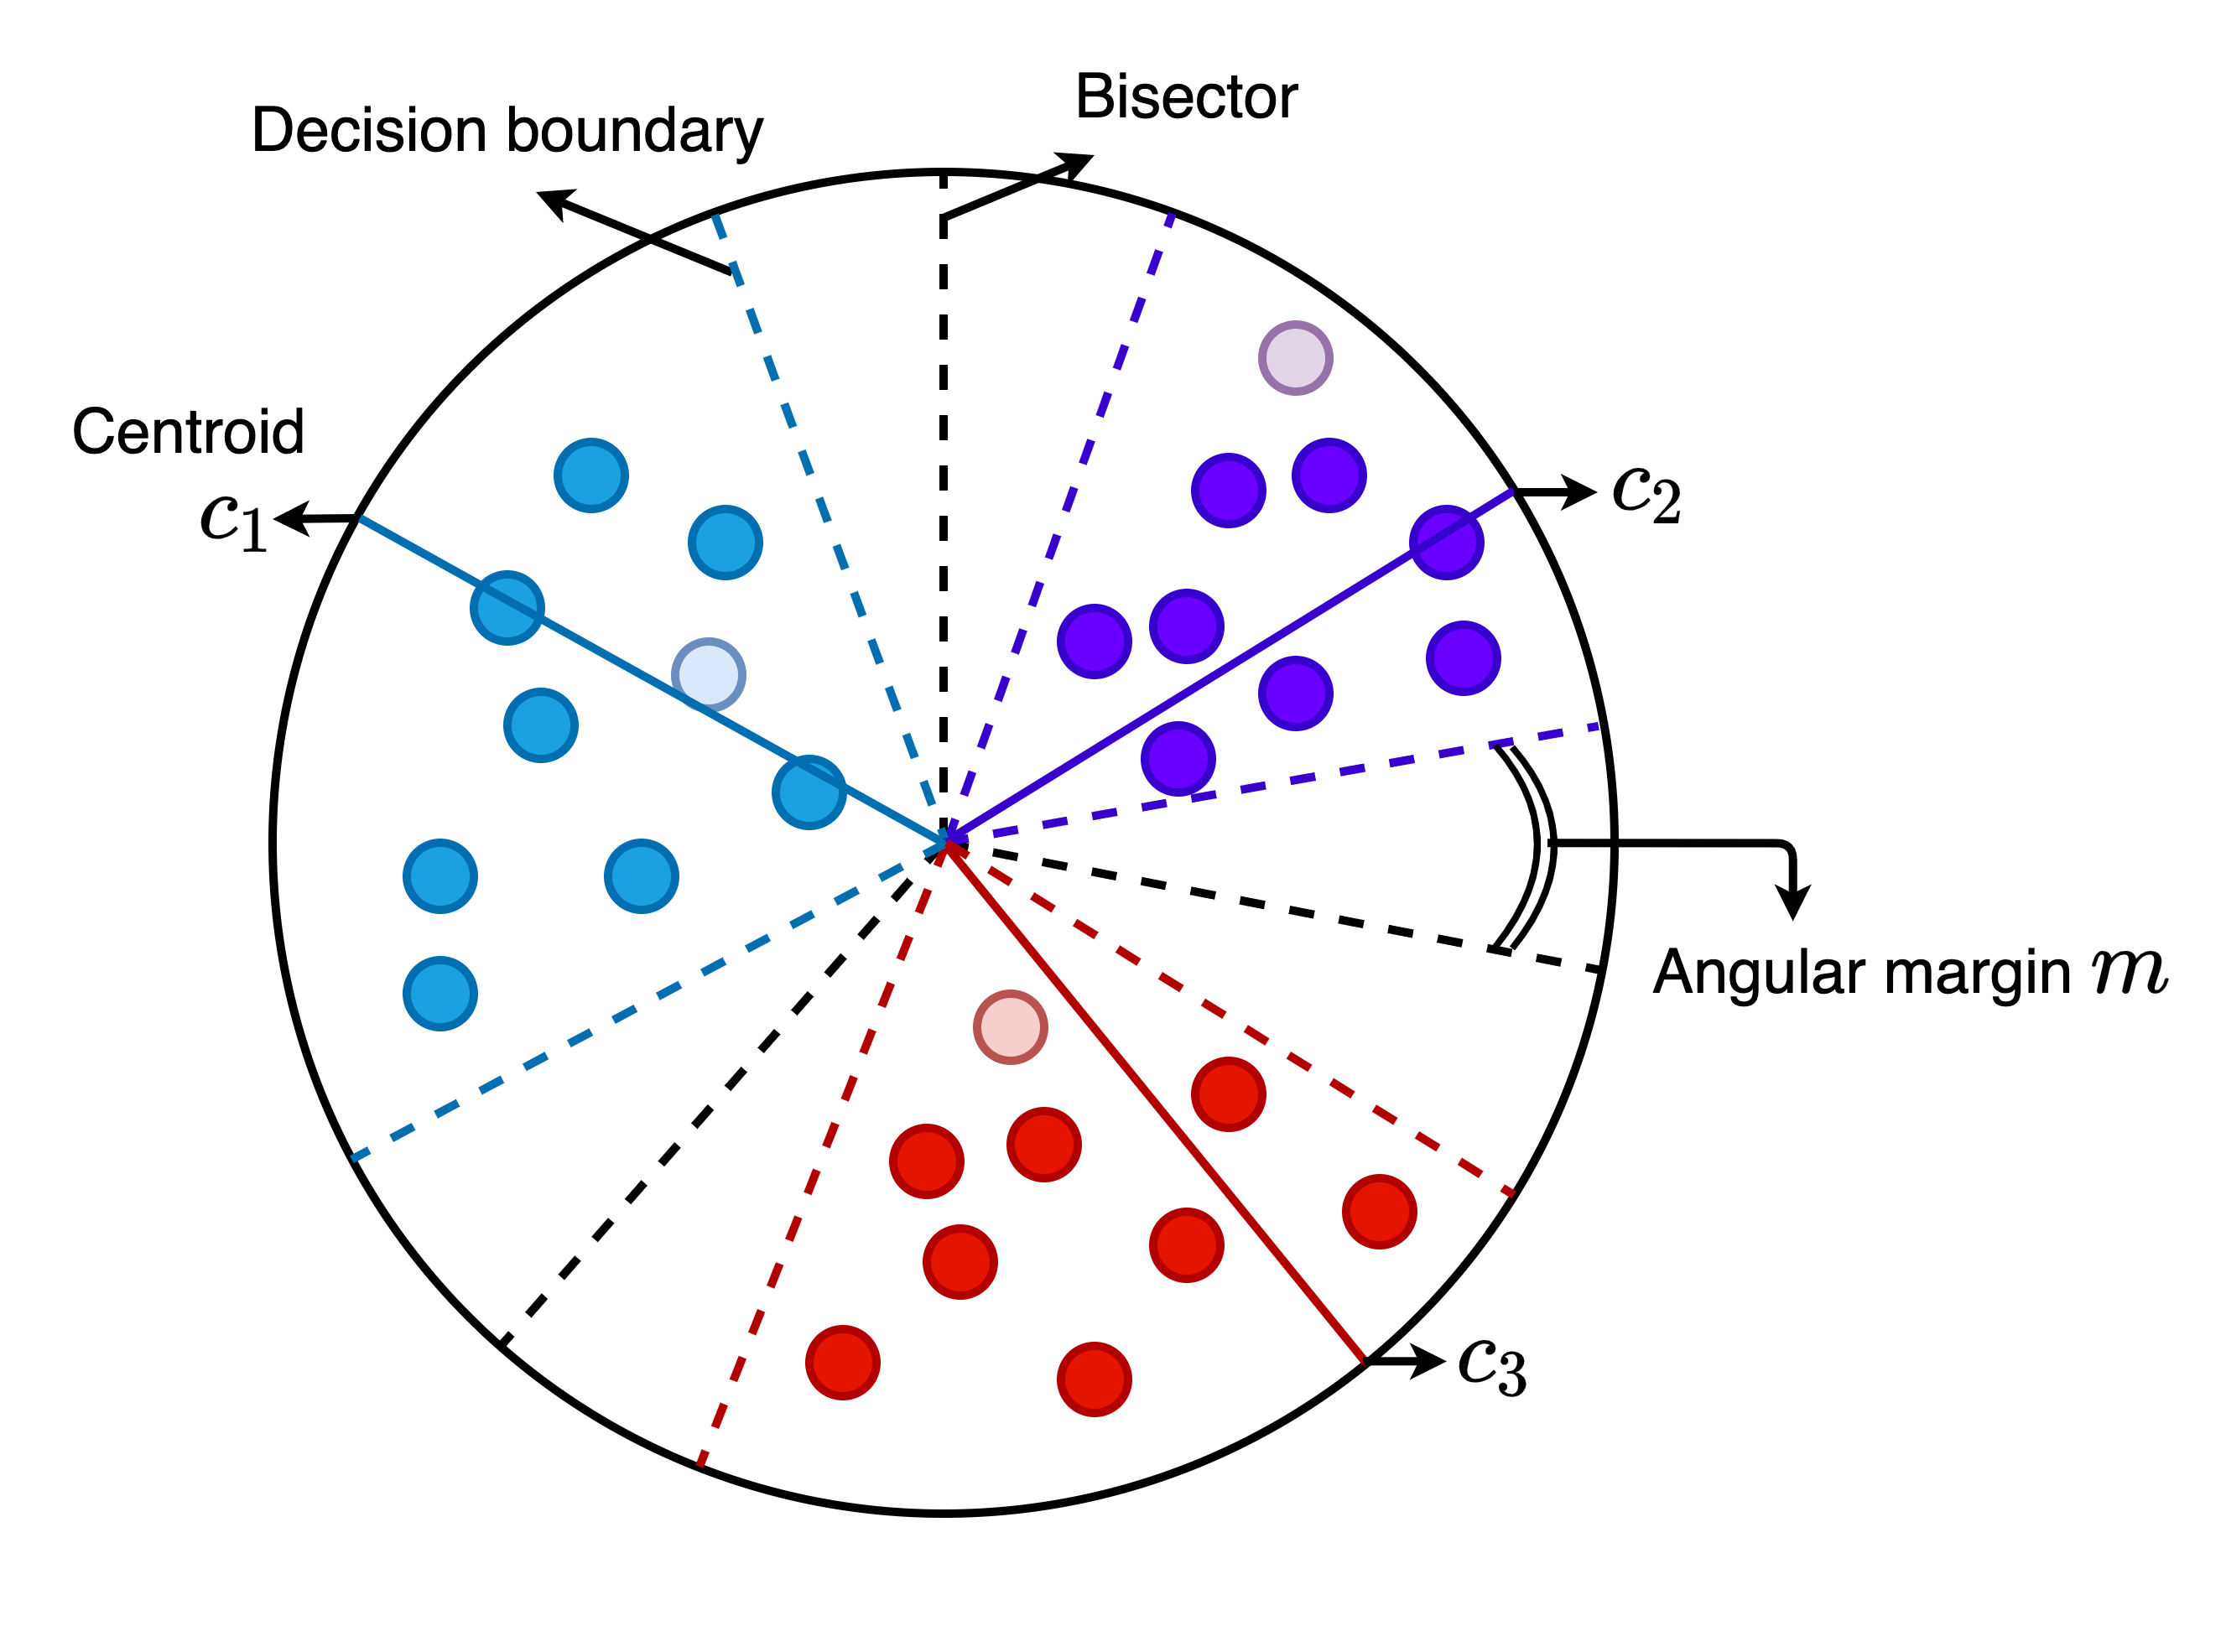
\includegraphics[width=0.65\textwidth]{images/margin-angular-space.png}
    \caption{Mô tả biểu diễn người nói học bởi hàm AMP-arc trong không gian góc.}
    \label{fig:margin-angular-space}
\end{figure}

Sự co cụm của các câu người nói (intra-class compactness) và khoảng cách với các người nói khác (inter-class separability) là 2 yếu tố chính đóng góp cho khả năng phân biệt biểu diễn người nói trong không gian vec-tơ. Việc thêm hệ số phạt lề trực tiếp làm tăng khoảng cách giữa các người nói và gián tiếp làm co cụm vùng biểu diễn của một người (Hình \ref{fig:margin-angular-space}). 

Theo các tác giả của hàm ArcFace \cite{deng2019arcface}, thiết kế hệ số phạt theo các cách khác nhau có ảnh hưởng rất lớn trong quá trình huấn luyện mô hình. Hàm AMP-arc lấy cảm hứng từ hàm ArcFace có thuộc tính hình học tốt hơn hàm AMP-cos do nó có sự tương ứng chính xác với khoảng cách trong không gian góc. Hình \ref{fig:arcface} cho thấy trong trường hợp phân loại nhị phân, hàm arc biên quyết định tuyến tính trong toàn không gian trong khi hàm cos có biên quyết định phi tuyến tính.

\begin{figure}[h]
    \centering
    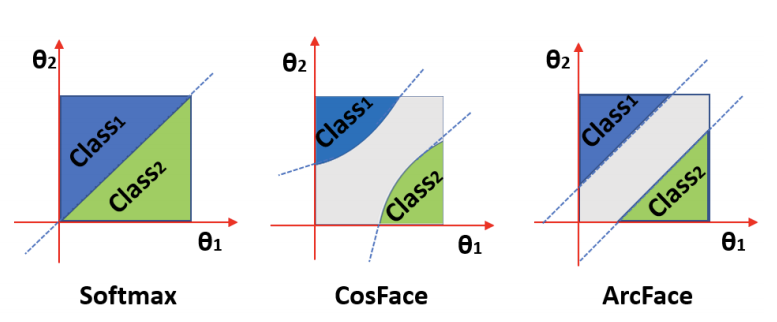
\includegraphics[width=0.65\textwidth]{images/arcface.png}
    \caption{Biên quyết định của các hàm khác nhau trong phân loại nhị phân \cite{schroff2015facenet}.}
    \label{fig:arcface}
\end{figure}

\section{Nghiên cứu liên quan}
% \section{Các nghiên cứu học sâu giải quyết bài toán nhận diện giọng nói}
\label{related-works}

Các mô hình học sâu hiện đại giải quyết bài toán nhận diện giọng nói thường gồm ba phần chính (Hình \ref{fig:model-architecture}):

\begin{itemize}
    \item Một mạng nơ-ron làm công cụ trích xuất biểu diễn người nói cho một khung đặc trưng tiếng nói.
    \item Lớp tổng hợp dữ liệu: lớp này sử dụng biểu diễn của các khung âm thanh từ mạng nơ-ron để tổng hợp ra một vec-tơ duy nhất đại diện cho đoạn tiếng nói đầu vào.
    \item Một hàm mất mát để tối ưu toàn bộ mô hình.
\end{itemize}

\begin{figure}[h]
    \centering
    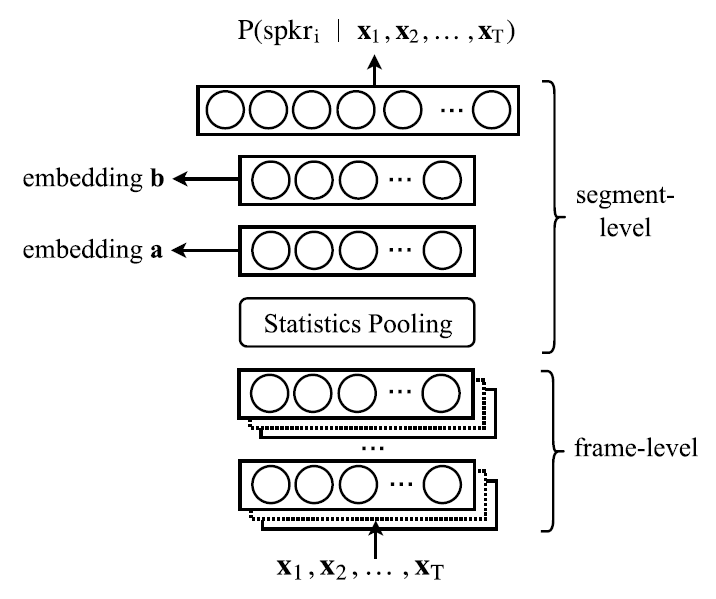
\includegraphics[width=0.8\textwidth]{images/x-vector.png}
    \caption{Tổng quan mô hình nhận diện người nói \cite{snyder2018x}}
    \label{fig:model-architecture}
\end{figure}

Trong pha kiểm tra, mạng nơ-ron và lớp tổng hợp dữ liệu được sử dụng để tạo ra vec-tơ biểu diễn của đoạn tiếng nói kiểm tra. Hàm mất mát chỉ được sử dụng trong pha phát triển, và bị loại bỏ trong pha kiểm tra và pha ghi danh.

Phần lớn các nghiên cứu về nhận dạng người nói hướng tới cải thiện hệ thống qua nâng cao hiệu quả của lớp tổng hợp dữ liệu và hàm mất mát. Về mạng nơ-ron trích xuất đặc trưng, các nghiên cứu chủ yêu sử dụng các mạng xương sống thành công trong các bài toán khác như phân loại hình ảnh (Ví dụ: mạng VGG \cite{simonyan2014very} và mạng ResNet \cite{he2016deep}) và nhận dạng tiếng nói (mạng TDNN \cite{waibel1989phoneme} và mạng LSTM \cite{hochreiter1997long}). 

Một vài nghiên cứu nổi bật cho lớp tổng hợp có thể kể đến như: tổng hợp trung bình (average pooling) \cite{variani2014deep}, tổng hợp thống kê (statistical pooling) \cite{snyder2018x}, tổng hợp dựa trên cơ chế tập trung (attentive pooling) \cite{zhu2018self,okabe2018attentive}, hay mã hoá dựa trên từ điển NetVLAD/GhostVLAD trong \cite{xie2019utterance}.

Các nghiên cứu tiên phong \cite{variani2014deep, snyder2018x, snyder2017deep} ứng dụng mạng nơ-ron nhận tạo vào bài toán nhận dạng người nói học không gian biểu diễn bằng các hàm mất mát phân loại (classification loss). Trên cơ sở đó, các nghiên cứu thịnh hành \cite{okabe2018attentive, snyder2019speaker, ravanelli2018speaker} sử dụng hàm softmax để huấn luyện mô hình. Hàm softmax có khả năng học để phân loại người nói một cách hiêu quả, tuy nhiên, nó không được thiết kế để tối ưu tính tương đồng trong không gian biểu diễn. 

Để giải quyết điểm yếu của softmax, công trình của Liu và cộng sự \cite{liu2017sphereface} đề xuất hàm angular softmax (A-Softmax) cho bài toán nhận diện khuôn mặt bằng cách dùng độ tương đồng cô-sin làm đầu vào của hàm softmax. Các nghiên cứu sau đó áp dụng hàm A-Softmax trên bài toán nhận dạng người nói \cite{villalba2019state, snyder2019jhu} cho thấy sự vượt trội của hàm này so với softmax thông thường. Các phiên bản cải tiến của hàm A-Softmax như AM-Softmax \cite{wang2018additive} và AAM-Softmax \cite{deng2019arcface} sử dụng hàm phạt biên trở nên phổ biến cho bài toán nhận dạng người nói do dễ dàng cài đặt và hiệu năng cao. Tuy nhiên, huấn luyện mô hình với AM-Softmax và AAM-Softmax khá khó khăn do hai hàm này rất nhạy cảm với sự điều chỉnh tham số.

Bên cạnh nhóm hàm mục tiêu phân loại, học phân biệt cũng là lựa chọn phổ biến cho bài toán nhận dạng người nói. Thay vì phân loại, mục tiêu của học biểu diễn là tối ưu không gian biểu diễn \ref{fig:metric-learning}. Trong bài toán nhận dạng người nói, biểu diễn của các câu nói từ cùng một người được kéo lại gần nhau trong không gian biểu diễn, ngược lại câu của những người khác nhau bị đẩy ra xa. 

\begin{figure}[h]
    \centering
    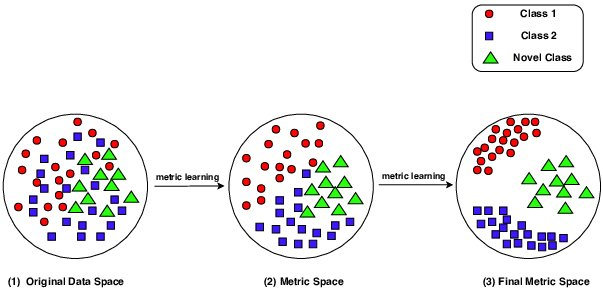
\includegraphics[width=0.9\textwidth]{images/metric-learning.jpg}
    \caption{Không gian biểu diễn với học phân biệt\cite{wang2019metric}}
    \label{fig:metric-learning}
\end{figure}

Hai hàm học biểu diễn nổi tiếng là contrastive loss \cite{chopra2005learning} và triplet loss \cite{schroff2015facenet} xuất phát từ bài toán nhận diện khuôn mặt cho kết quả hứa hẹn trong bài toán nhận diện người nói \cite{zhang2018text,rahman2018attention}.Năm 2020, Chung và cộng sự \cite{chung2020defence} đề xuất hàm Angular Prototypical cho kết quả vượt trội khi so với các hàm mục tiêu phân loại. 
% \TODO{prototypical, GE2E}. 

% https://medium.com/analytics-vidhya/exploring-other-face-recognition-approaches-part-2-arcface-88cda1fdfeb8
% https://medium.com/analytics-vidhya/exploring-other-face-recognition-approaches-part-1-cosface-4aed39afe7a8